\section{APRENDIZAJE PROFUNDO}
    Buscando resolver el problema de la generalización e invarianza a los datos de los que sufren muchos modelos de machine learning o aprendizaje automático, es que nace el Deep Learning o aprendizaje profundo el cual propone apilar múltiples capas con varias neuronas cada una en una red neuronal para lograr representar funciones más complejas y altamente no lineales, a cambio de requerir muchos más datos para su entrenamiento. \citep{Goodfellow-et-al-2016}
    \subsection{PERCEPTRÓN MULTICAPA}
        El perceptrón multicapa, más conocido como red neuronale, extiende la idea de la regresión logística y lineal a un modelo de $n$-etapas, una especie de concatenación de regresiones con la diferencia que a la salida de las capas se les aplica una función $g(\mathbf{X})$ denominada función de activación, que consiste en alguna transformación no lineal de las variables de salida intermedias con el fin de poder realizar ajustes más complejos a los datos. \citep{hastie01statisticallearning}
        
        \begin{figure}[h]
            \centering
            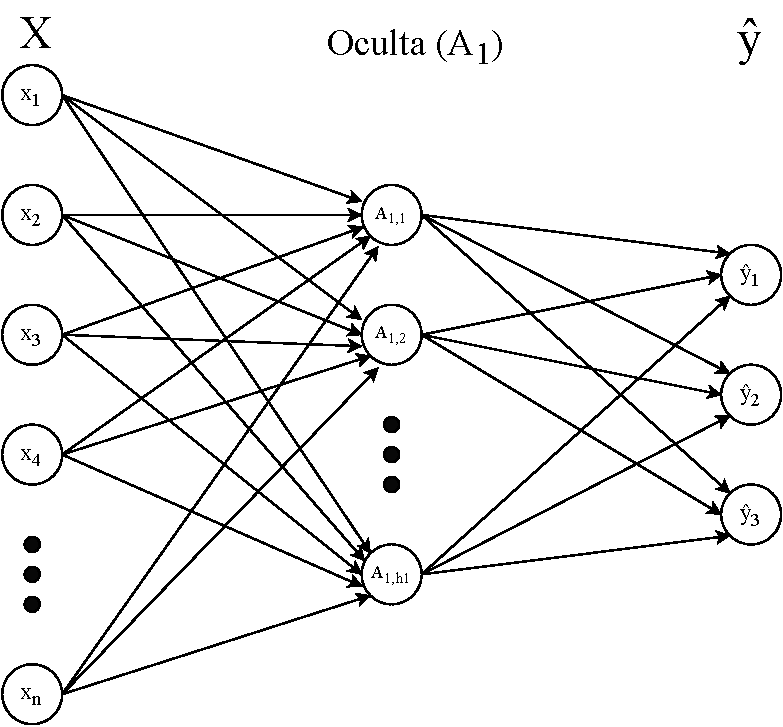
\includegraphics[scale=0.55]{imagenes/NeuralNetwork}
            \caption{Red neuronal con una capa oculta\\Fuente: elaboración propia}
        \end{figure}
        % \vspace{-8mm}
        % \begin{center}
            % Fuente: elaboración propia
        % \end{center}  
        
        Conforme aumentamos la cantidad de capas y parámetros de una red neuronal, esta puede aproximar funciones cada vez más complejas, por lo que se le denomina un aproximador universal de funciones, ya que el espacio $\mathcal{H}$ de todas las posibles funciones que puede aproximar, es infinito, es debido a esto que se requieren más observaciones en la muestra de la distribución de datos a modelar. \citep{Goodfellow-et-al-2016}
        
        La red neuronal matemáticamente es una composición de $n$ funciones o capas, aplicando una no linealidad $g(\mathbf{X})$ en cada etapa, con una función de enlace $g(\mathbf{X})$ en la capa de salida, la cual comúnmente es una softmax para clasificación o la identidad para regresión, siendo esta última etapa una regresión logística o lineal respectivamente, con variables de entrada procesadas por las anteriores capas de manera que sea linealmente aproximable en un número arbitrario de dimensiones elegidas por el modelo al entrenarse sobre los datos. La función de costo se denota por $J(\theta)$ con $\theta$ todos los parámetros del modelo. \citep{bishop}
        
        \begin{equation}
        \begin{aligned}
            Z_1 &= X \cdot W_1 + b_1\\
    		A_1 &= g_1(Z_1) \\
    		Z_2 &= A_1 \cdot W_2 + b_2 \\
    		A_2 &= g_2(Z_2) \\
    		&\vdots\\
    		Z_n &= A_{n-1} \cdot W_n + b_n\\
    		\hat{Y} &= h(Z_n) \\
    		J(\theta) &= \sum_{i}^{m} \mathcal{L}(\hat{y_i}, y_i)
        \end{aligned}
        \end{equation}
        
        Basándonos en la definición de la matriz $\mathbf{X}$ descrita en el modelo de regresión lineal, la columna de unos agregada antes de ajustar el modelo para el parámetro constante, ahora se considerará como un vector de parámetros $b_k$ para las $l_k$ neuronas de la capa $k$, y los demás parámetros son representados por la matriz $W_k$.
        
        \subsubsection{FUNCIONES DE ACTIVACIÓN}
        Con el fin de obtener aproximaciones no lineales a los datos, se debe evaluar la salida $Z_k$ de cada capa en una función de activación no lineal $g_k(Z_k)$.
        
        Las funciones de activación más comúnmente usada por ser fácil de computar y diferenciar es la \textit{Rectified Linear Unit} o \textbf{RELU} \citep{Goodfellow-et-al-2016}, la cual está definida por:
        \begin{equation}
            g(Z_k) = max(0, Z_k) \text{ $\forall$ $z_{k,j}$ / $j$ : $0, 1, ..., l_k$}
        \end{equation}
        
        \noindent cuya derivada con fines de estabilidad numérica es
        
        \begin{equation}
			\frac{\partial g(Z_k)}{\partial Z_k} = 
			\begin{cases}
			\text{1 si } z_{k,j} > 0\\
			\text{0 en otro caso}
			\end{cases}
		\end{equation}
        
        \subsubsection{RETROPROPAGACIÓN DE LOS ERRORES}
        Para ajustar los parámetros o entrenar la red neuronal, al tener más capas por las que pasar para obtener todos los gradientes de los errores, debemos derivar a través de cada una de ellas, a este algoritmo se le llama Backpropagation o Retropropagación, que es simplemente como su nombre dice, propagar los gradientes de reverso a través de la red neuronal.
		
		Primero se obtiene la derivada con respecto da cada uno de los parámetros de la composición de funciones por regla de la cadena
		
		\begin{equation}
		    \frac{\partial J}{\partial \theta_k} = \frac{\partial J}{\partial Z_n} \cdot  \frac{\partial Z_{n}}{\partial A_{n-1}} \cdot \frac{\partial A_{n-1}}{\partial Z_{n-1}} \cdot  \dots \cdot \frac{\partial A_{k}}{\partial Z_{k}} \cdot \frac{\partial Z_{k}}{\partial \theta_{k}}
		\end{equation}
		
		\noindent dónde $\theta_k$ representa cualquiera de los parámetros de $W_k$ o $b_k$ en la capa $k$, notese que para obtener la derivada con respecto de los parámetros en la capa $k$ se requiere la derivada en con respecto de las activaciones las capas siguientes, así, cuando obtenemos la derivada con respecto de los parámetros de la capa $k$ ya calculamos para todas las capas siguientes y sólo debemos multiplicar por la derivada de la salida lineal de la capa $k$ con respecto del parámetro $\theta_k$. \citep{bishop}
		
		Para el caso de regresión y clasificación con softmax $\frac{\partial J}{\partial Z_n} = (\mathbf{\hat{Y}} - \mathbf{Y})$ de forma vectorial, de manera general la derivada con respecto de algún parámetro está dada por
		
		\begin{equation}
		    \frac{\partial J}{\partial \theta_k} = \frac{\partial J}{\partial Z_n} \cdot \prod_{i=0}^{n-(k+1)} W_{n-i} \frac{\partial g_{n-(i+1)}(Z_{n-(i+1)})}{\partial Z_{n-(i+1)}} \cdot \frac{\partial Z_k}{\partial \theta_k}
		\end{equation}
		
		Similar a la regresión logística, se estiman los parámetros mediante un método de optimización, cuyo requisito sea la derivada con respecto a cada uno de los parámetros.
		
    \subsection{REDES NEURONALES CONVOLUCIONALES}
        Es un tipo de arquitectura de redes neuronales diseñada específicamente para tareas sobre imágenes, de manera que las operaciones sobre las observaciones de entrada ya no son composiciones realizando multiplicaciones matriciales, sino que cada neurona se convierte en un filtro o kernel de dimensiones $(k \times k)$, de los cuales tenemos varios filtros que se aplican sobre la imagen mediante la convolución.
        
        \begin{figure}[H]
            \centering
            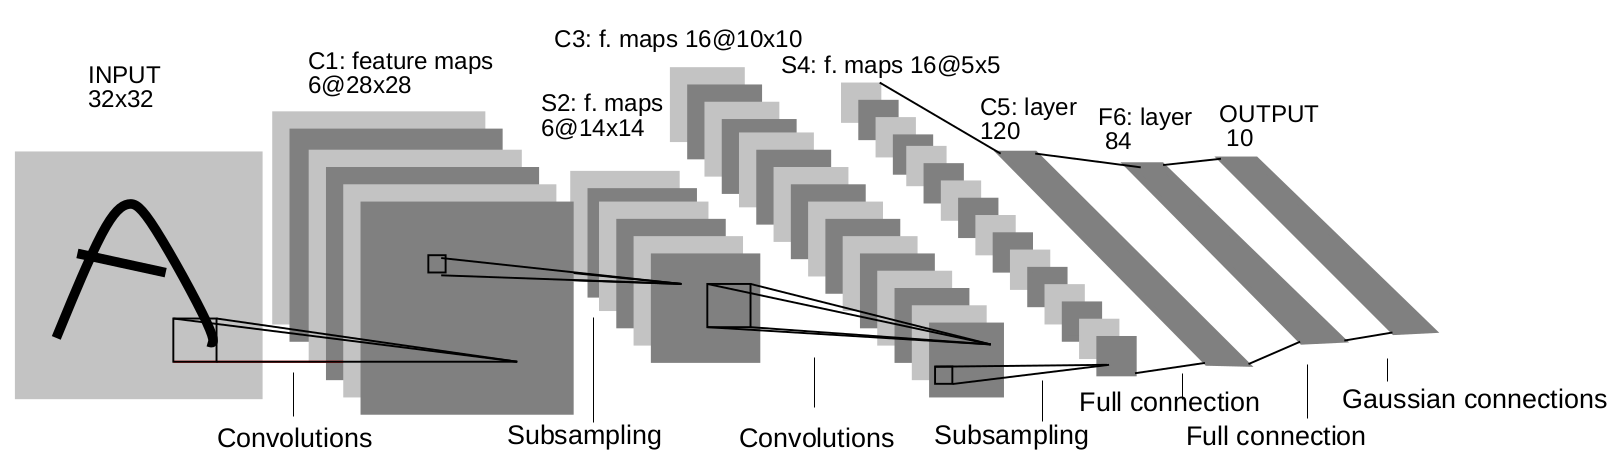
\includegraphics[scale=0.25]{imagenes/lenet}
            \caption{Red neuronal convolucional para la clasificación de dígitos manuscritos\\ Fuente: \citep{lecun-gradientbased-learning-applied-1998}}
        \end{figure}
        % \vspace{-8mm}
        % \begin{center}
        %     Fuente: \citep{lecun-gradientbased-learning-applied-1998}
        % \end{center}
        La idea detrás de este tipo de red es que se apliquen varios filtros en cada capa de la red para extraer características importantes de los objetos que se buscan, estos filtros se aprenden mediante retropropagación y ya no se diseñan a mano \citep{Goodfellow-et-al-2016}.
        \subsubsection{STRIDES}
        Cuando se desea optimizar la operación sacrificando representabilidad o disminuir la muestra, se puede incrementar el tamaño del salto de la ventana deslizante al convolucionar la imágen con el filtro, a este salto se le llama \textbf{stride}
        
        
        Aplicando esta idea, se obtiene una fórmula general para calcular la dimensión de la matriz resultante al aplicar cada uno de los filtros con un stride $s$
        
        $$\frac{I_{alto} - k + s}{s} \times \frac{I_{ancho} - k + s}{s}$$ 
        
        \begin{figure}[H]
            \centering
            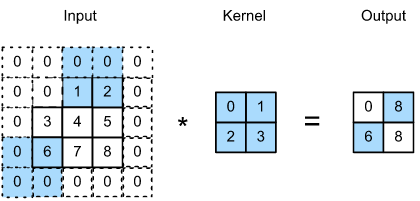
\includegraphics[scale=0.6]{imagenes/stride}
            \caption{Convolución con $s=2$\\ Fuente: \citep{zhang2020dive}}
        \end{figure}
        % \vspace{-8mm}
        % \begin{center}
        %     Fuente: \citep{zhang2020dive}
        % \end{center}
        \subsubsection{POOLING}
        Es una operación sobre la entrada bidimensional que con un stride $s$ recorre una ventana deslizante de dimensión $p \times p$ extrayendo información característica de cada sección de la entrada.
        
        Existen dos tipos de pooling más comunes, average pooling que promedia los valores activados en cada sección de la imágen sobre la que pasa la ventana y max pooling, el cual extrae el elemento más representativo, es decir el con mayor valor, de cada sección de la imágen.
        
        \begin{figure}[H]
            \centering
            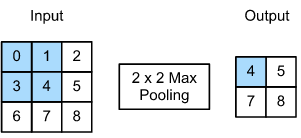
\includegraphics[scale=0.6]{imagenes/pooling}
            \caption{Pooling con con $s=1$\\ Fuente: \citep{zhang2020dive}}
        \end{figure}
        % \vspace{-8mm}
        % \begin{center}
        %     Fuente: \citep{zhang2020dive}
        % \end{center}
    \subsection{APRENDIZAJE DE REPRESENTACIONES PROFUNDAS}
    En cada etapa de la red neuronal se extraen características representativas de la imagen que ayuden a realizar la predicción de la tarea para la cual se la entrena, conforme pasan más etapas en la red los filtros buscan características más específicas \citep{Goodfellow-et-al-2016}
    
    \begin{figure}[H]
            \centering
            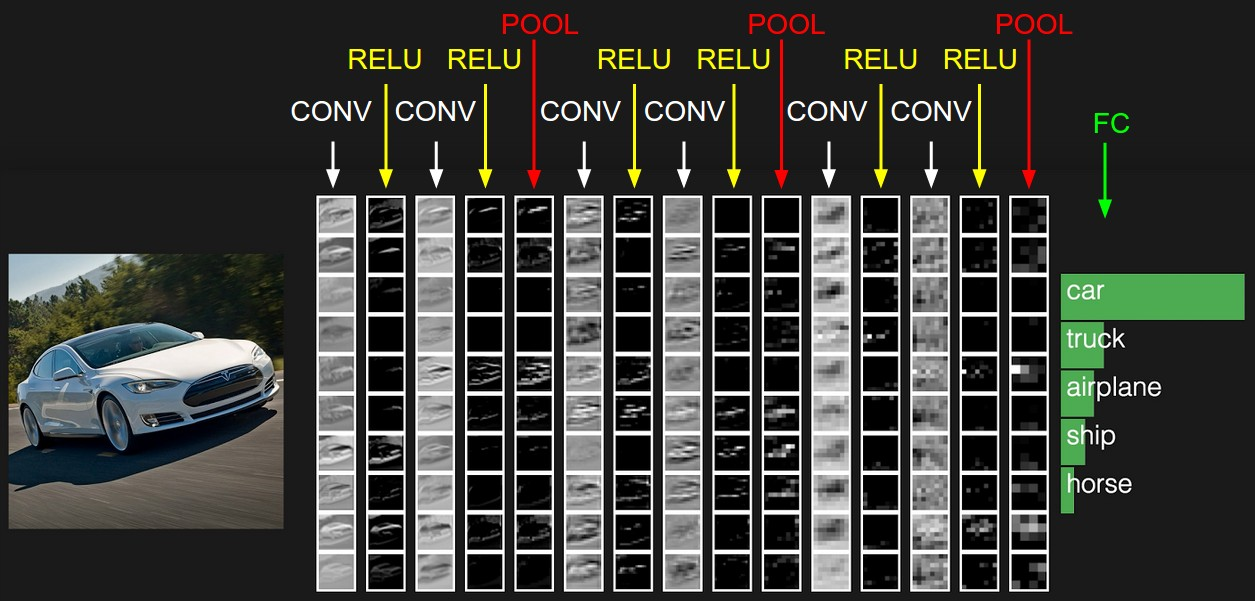
\includegraphics[scale=0.3]{imagenes/convnet}
            \caption{Extracción de las características profundas aprendidas\\ Fuente: \citep{stanford_2020}}
        \end{figure}
        % \vspace{-8mm}
        % \begin{center}
        %     Fuente: \citep{stanford_2020}
        % \end{center}
    
    \noindent de esta manera activando (dando valores altos) a ciertas partes de la imagen que es donde ``presta atención'' en busca de los objetos que desee clasificar o en base a los que predecir algún valor numérico

    \begin{figure}[H]
            \centering
            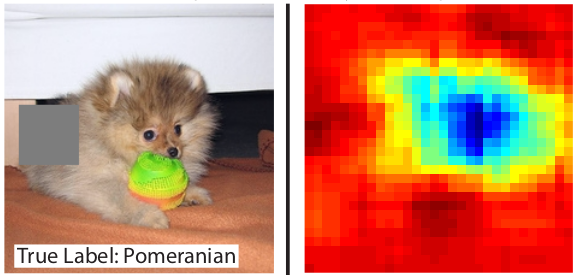
\includegraphics[scale=0.5]{imagenes/activation_cnn}
            \caption{Activación de los píxeles de la imagen en la $5^{ta}$ capa de la red\\ Fuente: \citep{10.1007/978-3-319-10590-1_53}}
        \end{figure}
        % \vspace{-8mm}
        % \begin{center}
        %     Fuente: \citep{10.1007/978-3-319-10590-1_53}
        % \end{center}
    \noindent a esto se le llama aprendizaje de representaciones profundas, porque los filtros aprenden información desde bajo a alto nivel que caracterice los objetos en las etiquetas de entrenamiento. 
